\chapter{经典力学的初步处理}\label{chap:first-classical-mechanics}

在本章中,我们用一种相当初等的方式回顾经典力学.虽然这里的内容对物理学家来说可能显得过于基础,但它为后面讨论量子力学提供了必要的语言和动机.

\section{一维运动}

\subsection{牛顿定律}

先考虑在实轴 $\mathbb{R}^{1}$ 上运动的粒子.设粒子在时刻 $t$ 的位置为 $x(t)$,速度为 $\dot{x}(t)$,加速度为 $\ddot{x}(t)$,质量为 $m$.牛顿第二定律说,粒子的加速度与所受力 $F$ 成正比:

\begin{equation}
  m\ddot{x}(t)=F\bigl(x(t)\bigr).
  \label{eq:newton-one-dimensional}
\end{equation}

这里我们首先假设力只依赖于位置,而不依赖于速度.牛顿三定律中,后面我们最常使用的是第二定律.由于方程~\eqref{eq:newton-one-dimensional} 是二阶方程,适当的初始条件(也就是得到唯一解所需要的条件)是在某个初始时刻 $t_{0}$ 给出位置和速度.因此,我们寻找满足

\[
  x(t_{0})=x_{0},\qquad \dot{x}(t_{0})=v_{0}
\]
的方程~\eqref{eq:newton-one-dimensional} 的解.

假设 $F$ 是光滑函数,常微分方程初等理论中的标准结果告诉我们:对每一组初始条件,都存在唯一的局部解.这里的“局部解”是指定义在初始时刻 $t_{0}$ 的某个邻域内的解.由于方程~\eqref{eq:newton-one-dimensional} 一般是非线性的,所以不能期待任意力函数对应的解都对所有 $t$ 存在.例如,若 $F(x)=x^{2}$,那么任何具有正初始位置和正初始速度的解都会在有限时间内逃向无穷远(将练习~\ref{ex:repelling-potential} 应用于 $V(x)=-x^{3}/3$ 即可).关于存在性和唯一性的证明,参见 [28] 中的例题 8.2 和定理 8.13.

\begin{definition}[轨迹]\label{def:trajectory}
方程~\eqref{eq:newton-one-dimensional} 的一个解 $x(t)$ 称为一条\emph{轨迹}.
\end{definition}

\begin{example}[谐振子]\label{ex:harmonic-oscillator}
如果力由 Hooke 定律给出,即 $F(x)=-kx$,其中 $k$ 是正数,那么牛顿定律可以写成
\[
  m\ddot{x}+kx=0.
\]
这个方程的通解为
\begin{equation}
  x(t)=a\cos(\omega t)+b\sin(\omega t),
  \qquad \omega:=\sqrt{\frac{k}{m}},
  \label{eq:harmonic-oscillator-solution}
\end{equation}
其中 $\omega$ 是振荡频率.
\end{example}

例题~\ref{ex:harmonic-oscillator} 中的系统称为(经典)谐振子.它可以描述一个连接在弹簧上的质量块:力与弹簧相对于平衡位置的伸长量 $x$ 成正比.$-kx$ 前面的负号表示力会把振子拉回平衡位置.这里以及本书其他地方,我们使用“角频率”的概念,即正弦或余弦函数的自变量变化率.如果 $\omega$ 是角频率,那么“普通”频率——即单位时间内完成的周期数——为 $\omega/(2\pi)$.说 $x$ 具有(角)频率 $\omega$,意味着 $x$ 的周期为 $2\pi/\omega$.

\subsection{能量守恒}

现在回到一般的力函数 $F(x)$.我们把系统的动能定义为 $\frac12mv^{2}$,并把系统的势能定义为

\begin{equation}
  V(x)=-\int F(x)\,\mathrm{d}x,
  \label{eq:potential-one-dimensional}
\end{equation}

于是 $F(x)=-\mathrm{d}V/\mathrm{d}x$.(势能只确定到加上一个常数为止.)系统的总能量为

\begin{equation}
  E(x,v)=\frac12mv^{2}+V(x).
  \label{eq:energy-one-dimensional}
\end{equation}

能量函数的主要意义在于它是守恒的,也就是说,它沿任意轨迹取恒定值.

\begin{theorem}[能量守恒]\label{thm:one-dimensional-energy}
设粒子满足形式为 $m\ddot{x}=F(x)$ 的牛顿定律,并令 $V$ 和 $E$ 分别如式~\eqref{eq:potential-one-dimensional} 与~\eqref{eq:energy-one-dimensional} 所定义.那么能量 $E$ 守恒:对牛顿定律的每一个解 $x(t)$,$E\bigl(x(t),\dot{x}(t)\bigr)$ 都与 $t$ 无关.
\end{theorem}

\begin{proof}
利用链式法则直接求导:
\begin{align*}
\frac{\mathrm{d}}{\mathrm{d}t}E\bigl(x(t),\dot{x}(t)\bigr)
 &=\frac{\mathrm{d}}{\mathrm{d}t}\left(\frac12m\dot{x}(t)^{2}+V\bigl(x(t)\bigr)\right)\\
 &=m\dot{x}(t)\ddot{x}(t)+\frac{\mathrm{d}V}{\mathrm{d}x}\dot{x}(t)\\
 &=\dot{x}(t)\left[m\ddot{x}(t)-F\bigl(x(t)\bigr)\right].
\end{align*}
最后一个表达式由牛顿定律为零.因此,能量沿任意轨迹的时间导数为零,从而 $E\bigl(x(t),\dot{x}(t)\bigr)$ 与 $t$ 无关.
\end{proof}

我们也可以把能量称为一个守恒量(或运动常数),因为粒子按照牛顿定律运动时既不会获得能量,也不会失去能量.

让我们看看能量守恒如何帮助我们理解牛顿定律的解.只需把速度 $v$ 作为新的变量引入,就可以把二阶方程 $m\ddot{x}=F(x)$ 化为一对一阶方程.也就是说,我们寻找满足下列方程组的函数对 $(x(t),v(t))$:

\begin{equation}
  \frac{\mathrm{d}x}{\mathrm{d}t}=v(t),\qquad
  \frac{\mathrm{d}v}{\mathrm{d}t}=\frac{1}{m}F\bigl(x(t)\bigr).
  \label{eq:first-order-newton}
\end{equation}

如果 $(x(t),v(t))$ 是这个方程组的解,那么只要在第二个方程中用 $\mathrm{d}x/\mathrm{d}t$ 代替 $v$,就能立即看出 $x(t)$ 满足牛顿定律.粒子在 $\mathbb{R}^{1}$ 中运动时,所有可能的 $(x,v)$ 所成的集合(即 $\mathbb{R}^{2}$)称为粒子的\emph{相空间}.这个一阶方程组的适当初始条件是 $x(0)=x_{0}$ 与 $v(0)=v_{0}$.

一旦在相空间中工作,我们就可以利用能量守恒.能量守恒意味着,方程组~\eqref{eq:first-order-newton} 的每条解都必须完全位于能量函数的一条“等值曲线”上,即集合

\begin{equation}
  \left\{(x,v)\in\mathbb{R}^{2}:E(x,v)=E(x_{0},v_{0})\right\}.
  \label{eq:energy-level-curve}
\end{equation}

如果 $F$(因而 $V$)是光滑的,那么 $E$ 是 $x$ 和 $v$ 的光滑函数.只要~\eqref{eq:energy-level-curve} 不包含 $E$ 的临界点,根据隐函数定理,这个集合就是 $\mathbb{R}^{2}$ 中的一条光滑曲线.如果这个等值集还是一条简单闭曲线,那么方程的解就会沿着这条曲线不断绕行.因此,解在相空间中所描出的集合,仅仅利用能量守恒就可以确定.此时唯一尚未显现的是:这条曲线如何由时间参数化.

在力学中,能量这样的守恒量通常称为一个“运动积分”.之所以这样称呼,是因为虽然一维牛顿第二定律是关于 $x$ 的二阶方程,但能量只依赖于 $x$ 和 $\dot{x}$,而不依赖于 $\ddot{x}$.因此,若 $E_{0}$ 是粒子在时刻 $t_{0}$ 的能量,则方程
\[
  \frac{m}{2}\dot{x}(t)^{2}+V\bigl(x(t)\bigr)=E_{0}
\]
实际上是一个一阶微分方程.解出 $\dot{x}$,可将它写成更标准的形式:

\begin{equation}
  \dot{x}(t)=\pm\sqrt{\frac{2\bigl(E_{0}-V(x(t))\bigr)}{m}}.
  \label{eq:energy-first-integral}
\end{equation}

这说明,利用能量守恒,我们已经把原来的二阶方程变成了一阶方程;也就是说,我们把原方程“积分”了一次,将 $\ddot{x}(t)=\cdots$ 形式的方程变成了 $\dot{x}(t)=\cdots$ 形式.方程~\eqref{eq:energy-first-integral} 是可分离变量的,并且可以或多或少地显式求解(见练习 1).

\subsection{带阻尼的系统}

到目前为止,我们考虑的力只依赖于位置.然而,通常也会考虑同时依赖于速度和位置的力.例如,对于阻尼谐振子,人们通常假设除了弹簧力之外,还存在一个与速度成正比的阻尼力(比如摩擦力).于是
\[
  F=-kx-\gamma\dot{x},
\]
其中 $k$ 仍是弹簧常数,$\gamma>0$ 是阻尼常数.$-\gamma\dot{x}$ 前面的负号反映了阻尼力的方向与速度相反,因此会使粒子减速.这个系统的运动方程为
\[
  m\ddot{x}+\gamma\dot{x}+kx=0.
\]

如果 $\gamma$ 较小,方程的解表现为衰减振荡,即正弦和余弦函数乘以一个衰减指数;如果 $\gamma$ 较大,解则是纯粹的衰减指数(见练习 5).

对于阻尼谐振子,不再存在守恒能量.更确切地说,在 $\mathbb{R}^{2}$ 上不存在非常数连续函数 $E$,使得对牛顿定律的每一条解,$E(x(t),\dot{x}(t))$ 都与 $t$ 无关.要看出这一点,只需注意:当 $\gamma>0$ 时,所有解 $x(t)$ 都满足,当 $t$ 趋于无穷时,平面上的点 $(x(t),\dot{x}(t))$ 趋于原点.因此,如果 $E$ 连续且沿每条轨迹恒定,那么起点处的 $E$ 值必定等于原点处的 $E$ 值.

现在考虑一般的阻尼系统.

\begin{proposition}[阻尼系统中的能量]\label{pro:damped-energy}
设粒子所受的力满足
\[
  F(x,\dot{x})=F_{1}(x)-\gamma\dot{x},\qquad \gamma>0.
\]
定义系统的能量为
\[
  E(x,\dot{x})=\frac12m\dot{x}^{2}+V(x),
\]
其中 $\mathrm{d}V/\mathrm{d}x=-F_{1}(x)$.那么沿任意轨迹 $x(t)$,都有
\begin{equation}
  \frac{\mathrm{d}}{\mathrm{d}t}E\bigl(x(t),\dot{x}(t)\bigr)=-\gamma\dot{x}(t)^{2}\leq 0.
  \label{eq:damped-energy-decay}
\end{equation}
\end{proposition}

因此,虽然能量不守恒,但它随时间减小,这仍然给出了关于系统行为的一些信息.

\begin{proof}
按照定理~\ref{thm:one-dimensional-energy} 的证明方式求导,不过这一次 $\mathrm{d}V/\mathrm{d}x=-F_{1}(x)$:
\[
  \frac{\mathrm{d}}{\mathrm{d}t}E\bigl(x(t),\dot{x}(t)\bigr)
  =\dot{x}(t)\left[m\ddot{x}(t)-F_{1}\bigl(x(t)\bigr)\right].
\]
由于 $F_{1}$ 不是完整的力函数,方括号中的量不再是零,而是 $-\gamma\dot{x}$.因此 $\mathrm{d}E/\mathrm{d}t=-\gamma\dot{x}^{2}$.
\end{proof}

命题~\ref{pro:damped-energy} 可以这样理解:存在摩擦时,我们研究的系统会把一部分能量以热能的形式交给环境,所以系统自身的能量随时间下降.我们将会看到,在更高维空间中,即使力依赖于速度,只要这种力始终垂直于速度,能量仍然可能守恒.

\section{高维空间中的运动}

现在考虑在 $\mathbb{R}^{n}$ 中运动的粒子.粒子的位置 $x=(x_{1},\ldots,x_{n})$ 是 $\mathbb{R}^{n}$ 中的向量,速度 $v$ 和加速度 $a$ 也一样.记
\[
  \dot{x}=(\dot{x}_{1},\ldots,\dot{x}_{n})
\]
为 $x$ 关于 $t$ 的导数,并用 $\ddot{x}$ 表示 $x$ 的二阶导数.牛顿定律现在写成

\begin{equation}
  m\ddot{x}(t)=F\bigl(x(t),\dot{x}(t)\bigr),
  \label{eq:newton-n-dimensional}
\end{equation}

其中 $F:\mathbb{R}^{n}\times\mathbb{R}^{n}\to\mathbb{R}^{n}$ 是某个力函数,一般可以同时依赖于粒子的位置和速度.

我们先考虑与速度无关的力,并在这种情况下寻找守恒能量函数.

\begin{proposition}[高维中的能量守恒]\label{pro:n-dimensional-energy}
考虑方程~\eqref{eq:newton-n-dimensional},并假设力与速度无关,即 $m\ddot{x}(t)=F(x(t))$.那么,形如
\[
  E(x,\dot{x})=\frac12m\lvert\dot{x}\rvert^{2}+V(x)
\]
的能量函数守恒,当且仅当 $V$ 满足
\[
  -\nabla V=F,
\]
其中 $\nabla V$ 是 $V$ 的梯度.
\end{proposition}

这里说 $E$ “守恒”,是指对牛顿定律的每个解 $x(t)$,$E(x(t),\dot{x}(t))$ 都与 $t$ 无关.函数 $V$ 称为系统的势能.

\begin{proof}
求导得到
\begin{align*}
\frac{\mathrm{d}}{\mathrm{d}t}\left(\frac12m\lvert\dot{x}(t)\rvert^{2}+V(x(t))\right)
 &=m\sum_{j=1}^{n}\dot{x}_{j}(t)\ddot{x}_{j}(t)+\sum_{j=1}^{n}\frac{\partial V}{\partial x_{j}}\dot{x}_{j}(t)\\
 &=\dot{x}(t)\cdot\left[m\ddot{x}(t)+\nabla V\right]\\
 &=\dot{x}(t)\cdot\left[F(x)+\nabla V(x)\right].
\end{align*}
因此,对所有 $x$ 都有 $\mathrm{d}E/\mathrm{d}t=0$,当且仅当 $-\nabla V(x)=F(x)$.
\end{proof}

一维情形中,任意光滑函数都可以表示为另一个函数的导数;但在 $\mathbb{R}^{n}$ 中,并非每个向量值函数 $F(x)$ 都能表示为某个标量函数 $V$ 的负梯度.

\begin{definition}[保守力场]\label{def:conservative-field}
设 $F$ 是定义在区域 $U\subset\mathbb{R}^{n}$ 上的光滑、取值于 $\mathbb{R}^{n}$ 的函数.如果存在定义在 $U$ 上的光滑实值函数 $V$,使得 $F=-\nabla V$,则称 $F$ 是保守的.
\end{definition}

如果区域 $U$ 是单连通的,那么有一个简单的局部条件刻画保守函数.

\begin{proposition}[保守场的判定]\label{pro:conservative-field-test}
设 $U$ 是 $\mathbb{R}^{n}$ 中的单连通区域,$F$ 是定义在 $U$ 上的光滑、取值于 $\mathbb{R}^{n}$ 的函数.那么 $F$ 保守,当且仅当在 $U$ 的每一点都有
\begin{equation}
  \frac{\partial F_{j}}{\partial x_{k}}-\frac{\partial F_{k}}{\partial x_{j}}=0.
  \label{eq:conservative-field-test}
\end{equation}
\end{proposition}

当 $n=3$ 时,很容易验证条件~\eqref{eq:conservative-field-test} 等价于 $F$ 的旋度 $\nabla\times F$ 在 $U$ 上为零.单连通这一假设不能省略;见练习 7.

\begin{proof}
如果 $F$ 是保守的,那么
\[
  \frac{\partial F_{j}}{\partial x_{k}}
  =-\frac{\partial^{2}V}{\partial x_{k}\partial x_{j}}
  =-\frac{\partial^{2}V}{\partial x_{j}\partial x_{k}}
  =\frac{\partial F_{k}}{\partial x_{j}}
\]
在 $U$ 的每一点成立.反过来,如果 $F$ 满足~\eqref{eq:conservative-field-test},则可以沿路径对 $F$ 积分,并利用 Stokes 定理证明积分与路径的选择无关,从而得到 $V$.例如,$n=3$ 时可参见 [44] 第 549 页的定理 4.3.高维情形的证明完全相同,只要使用 Stokes 定理的一般形式即可.
\end{proof}

我们也可以考虑依赖于速度的力.例如,如果 $F(x,v)=-\gamma v+F_{1}(x)$,其中 $\gamma$ 是正数,那么能量仍会随时间减少.不过,在维数大于 1 时还会出现一种新现象:即使力依赖于速度,能量也可能守恒.

\begin{proposition}[垂直速度的力]\label{pro:velocity-perpendicular-force}
设 $\mathbb{R}^{n}$ 中的粒子受力为
\[
  F(x,v)=-\nabla V(x)+F_{2}(x,v),
\]
其中 $V$ 是光滑函数,并且 $F_{2}$ 满足
\begin{equation}
  v\cdot F_{2}(x,v)=0
  \label{eq:perpendicular-force}
\end{equation}
对所有 $x,v\in\mathbb{R}^{n}$ 成立.那么能量函数
\[
  E(x,v)=\frac12m\lvert v\rvert^{2}+V(x)
\]
沿每条轨迹恒定.
\end{proposition}

例如,如果 $F_{2}$ 是三维空间中磁场 $B(x)$ 施加在带电粒子上的力,那么
\[
  F_{2}(x,v)=qv\times B(x),
\]
其中 $q$ 是粒子的电荷;显然它满足条件~\eqref{eq:perpendicular-force}.

\begin{proof}
见练习 8.
\end{proof}

\section{粒子系统}\label{sec:particle-systems}

如果有一个由 $N$ 个粒子组成的系统,每个粒子都在 $\mathbb{R}^{n}$ 中运动,那么用
\[
  x^{j}=(x^{j}_{1},\ldots,x^{j}_{n})
\]
表示第 $j$ 个粒子的位置.因此,在 $x^{j}_{k}$ 中,上标 $j$ 表示第 $j$ 个粒子,下标 $k$ 表示第 $k$ 个分量.牛顿定律写成
\[
  m_{j}\ddot{x}^{j}=F^{j}\bigl(x^{1},\ldots,x^{N},\dot{x}^{1},\ldots,\dot{x}^{N}\bigr),
  \qquad j=1,2,\ldots,N,
\]
其中 $m_{j}$ 是第 $j$ 个粒子的质量.这里 $F^{j}$ 是作用在第 $j$ 个粒子上的力;一般来说,它不仅依赖于该粒子的位置和速度,也依赖于其他粒子的位置和速度.

\subsection{能量守恒}

在粒子系统中,我们不能期待每个单独粒子的能量都守恒,因为粒子相互作用时会交换能量.相反,在对力 $F^{j}$ 作适当假设后,我们应当能够为整个系统定义一个守恒能量函数,即系统的总能量.

考虑只依赖于粒子位置的力,并假设能量函数具有如下形式:
\begin{equation}
  E(x^{1},\ldots,x^{N},v^{1},\ldots,v^{N})
  =\sum_{j=1}^{N}\frac12m_{j}\lvert v^{j}\rvert^{2}+V(x^{1},\ldots,x^{N}).
  \label{eq:many-particle-energy}
\end{equation}
现在考察 $V$ 需要具有何种形式,才能使 $E$ 沿每条轨迹恒定.

\begin{proposition}[粒子系统的能量守恒]\label{pro:many-particle-energy}
形如~\eqref{eq:many-particle-energy} 的能量函数沿每条轨迹恒定,只要对每个 $j$ 都有
\begin{equation}
  \nabla_{j}V=-F^{j},
  \label{eq:many-particle-potential}
\end{equation}
其中 $\nabla_{j}$ 表示关于变量 $x^{j}$ 的梯度.
\end{proposition}

\begin{proof}
我们计算
\begin{align*}
\frac{\mathrm{d}E}{\mathrm{d}t}
 &=\sum_{j=1}^{N}\left[m_{j}\dot{x}^{j}\cdot\ddot{x}^{j}+\nabla_{j}V\cdot\dot{x}^{j}\right]\\
 &=\sum_{j=1}^{N}\dot{x}^{j}\cdot\left[m_{j}\ddot{x}^{j}+\nabla_{j}V\right]\\
 &=\sum_{j=1}^{N}\dot{x}^{j}\cdot\left[F^{j}+\nabla_{j}V\right].
\end{align*}
如果 $\nabla_{j}V=-F^{j}$,那么 $E$ 守恒.
\end{proof}

和单粒子情形一样,存在一个简单条件,能够判定是否存在满足~\eqref{eq:many-particle-potential} 的势函数 $V$.

\begin{proposition}[多粒子势函数的存在性]\label{pro:many-particle-potential-existence}
设力函数 $F=(F^{1},\ldots,F^{N})$ 定义在 $\mathbb{R}^{nN}$ 中的单连通区域 $U$ 上.那么存在定义在 $U$ 上的光滑函数 $V$,使得对所有 $j$ 都有 $\nabla_{j}V=-F^{j}$,当且仅当对所有 $j,k,l,m$ 都有
\begin{equation}
  \frac{\partial F^{j}_{k}}{\partial x^{l}_{m}}
  =\frac{\partial F^{l}_{m}}{\partial x^{j}_{k}}.
  \label{eq:many-particle-potential-test}
\end{equation}
\end{proposition}

\begin{proof}
将命题~\ref{pro:conservative-field-test} 应用于维数为 $nN$ 的空间,并将指标 $j,k$ 替换为二元组 $(j,k)$,将指标 $l,m$ 替换为二元组 $(l,m)$.
\end{proof}

\subsection{动量守恒}\label{subsec:many-particle-potentials}

现在引入粒子动量的概念.

\begin{definition}[动量]\label{def:momentum}
在 $N$ 粒子系统中,第 $j$ 个粒子的动量 $p^{j}$ 定义为该粒子质量与速度的乘积:
\[
  p^{j}=m_{j}\dot{x}^{j}.
\]
系统的总动量 $p$ 定义为
\[
  p=\sum_{j=1}^{N}p^{j}.
\]
\end{definition}

注意到
\[
  \frac{\mathrm{d}p^{j}}{\mathrm{d}t}=m_{j}\ddot{x}^{j}=F^{j}.
\]
因此,牛顿定律可以重新表述为:“力是动量的变化率.”这正是 Newton 最初表述第二定律的方式.

Newton 第三定律说:“对于每一个作用力,都存在一个大小相等、方向相反的反作用力.”当所有力都是“两粒子”类型并满足自然的对称性条件时,这条定律成立.所谓两粒子力,是指作用在第 $j$ 个粒子上的力 $F^{j}$ 可以写成各项 $F^{j,k}$($j\neq k$)之和,其中 $F^{j,k}$ 只依赖于 $x^{j}$ 和 $x^{k}$.相关的对称性条件是
\[
  F^{j,k}(x^{j},x^{k})=-F^{k,j}(x^{k},x^{j});
\]
也就是说,第 $j$ 个粒子施加在第 $k$ 个粒子上的力,等于第 $k$ 个粒子施加在第 $j$ 个粒子上的力的负值,即“大小相等、方向相反”.如果还假设这些力是保守的,那么系统的势能具有形式
\begin{equation}
  V(x^{1},x^{2},\ldots,x^{N})
  =\sum_{j<k}V^{j,k}(x^{j}-x^{k}).
  \label{eq:two-particle-potential}
\end{equation}

Newton 第三定律的一个重要后果是系统总动量守恒.

\begin{proposition}[总动量守恒]\label{pro:total-momentum}
假设对每个 $j$,作用在第 $j$ 个粒子上的力具有形式
\[
  F^{j}(x^{1},\ldots,x^{N})=\sum_{k\neq j}F^{j,k}(x^{j},x^{k}),
\]
并且满足“大小相等、方向相反”的条件
\[
  F^{j,k}(x^{j},x^{k})=-F^{k,j}(x^{k},x^{j}).
\]
那么系统的总动量守恒.
\end{proposition}

注意,由于 $p^{j}$ 的变化率是作用在第 $j$ 个粒子上的力 $F^{j}$,所以每个单独粒子的动量一般并不随时间保持不变;只有在平凡的无相互作用系统(所有力都为零)中才会如此.

\begin{proof}
求导得
\[
  \frac{\mathrm{d}p}{\mathrm{d}t}
  =\sum_{j=1}^{N}\frac{\mathrm{d}p^{j}}{\mathrm{d}t}
  =\sum_{j=1}^{N}F^{j}
  =\sum_{j=1}^{N}\sum_{k\neq j}F^{j,k}(x^{j},x^{k}).
\]
根据大小相等、方向相反的条件,$F^{j,k}(x^{j},x^{k})$ 与 $F^{k,j}(x^{k},x^{j})$ 两项相互抵消,所以 $\mathrm{d}p/\mathrm{d}t=0$.
\end{proof}

现在考虑一种更一般的情形:力是保守的,但不一定具有“两粒子”的形式.下面的结果表明,即使如此,动量仍然可能守恒.

\begin{proposition}[平移不变性与动量守恒]\label{pro:translation-momentum}
如果多粒子系统的力律来自势能 $V$,那么系统的总动量守恒,当且仅当
\begin{equation}
  V(x^{1}+a,x^{2}+a,\ldots,x^{N}+a)=V(x^{1},x^{2},\ldots,x^{N})
  \label{eq:translation-invariance-potential}
\end{equation}
对所有 $a\in\mathbb{R}^{n}$ 成立.
\end{proposition}

\begin{proof}
令 $a=te_{k}$,其中 $e_{k}$ 是第 $k$ 个位置为 1、其余位置为 0 的向量,将~\eqref{eq:translation-invariance-potential} 对 $t$ 求导并在 $t=0$ 处取值,得到
\[
  0=\sum_{j=1}^{N}\frac{\partial V}{\partial x^{j}_{k}}
  =-\sum_{j=1}^{N}F^{j}_{k}
  =-\sum_{j=1}^{N}\frac{\mathrm{d}p^{j}_{k}}{\mathrm{d}t}
  =-\frac{\mathrm{d}p_{k}}{\mathrm{d}t}.
\]
因此,如果~\eqref{eq:translation-invariance-potential} 成立,$p$ 就随时间保持不变.

反过来,如果动量守恒,那么在每个点上力的总和都为零.因此,对任意 $t$ 都有
\begin{align*}
\frac{\mathrm{d}}{\mathrm{d}t}V(x^{1}+ta,\ldots,x^{N}+ta)
 &=\sum_{j=1}^{N}\nabla_{j}V(x^{1}+ta,\ldots,x^{N}+ta)\cdot a\\
 &=-\left(\sum_{j=1}^{N}F^{j}(x^{1}+ta,\ldots,x^{N}+ta)\right)\cdot a\\
 &=0.
\end{align*}
所以被求导的量在 $t=0$ 和 $t=1$ 时取值相同,这就证明了~\eqref{eq:translation-invariance-potential}.
\end{proof}

这个结果的要旨是:动量守恒源于系统的平移不变性;这里的“平移不变性”是指同时将每个粒子平移相同的量后,系统保持不变.(关于这一结果的更一般形式,见练习 11.)如果势能具有两粒子形式~\eqref{eq:two-particle-potential},那么条件~\eqref{eq:translation-invariance-potential} 显然成立.

\subsection{质心}

现在讨论动量守恒的一个重要应用.

\begin{definition}[质心]\label{def:center-of-mass}
对一个在 $\mathbb{R}^{n}$ 中运动的 $N$ 粒子系统,在固定时刻,系统的质心是向量 $c\in\mathbb{R}^{n}$,定义为
\[
  c=\sum_{j=1}^{N}\frac{m_{j}}{M}x^{j},
\]
其中
\[
  M=\sum_{j=1}^{N}m_{j}
\]
是系统的总质量.
\end{definition}

质心是各粒子位置的加权平均.对 $c(t)$ 关于 $t$ 求导,得到
\begin{equation}
  \frac{\mathrm{d}c}{\mathrm{d}t}
  =\frac{1}{M}\sum_{j=1}^{N}m_{j}\dot{x}^{j}
  =\frac{p}{M},
  \label{eq:center-of-mass-velocity}
\end{equation}
其中 $p$ 是系统的总动量.

\begin{proposition}[质心的匀速直线运动]\label{pro:center-of-mass-motion}
假设系统的总动量 $p$ 守恒.那么质心沿直线以恒定速率运动.具体来说,
\begin{equation}
  c(t)=c(t_{0})+(t-t_{0})\frac{p}{M},
  \label{eq:center-of-mass-line}
\end{equation}
其中 $c(t_{0})$ 是某个初始时刻 $t_{0}$ 的质心.
\end{proposition}

\begin{proof}
结论直接由式~\eqref{eq:center-of-mass-velocity} 得出.
\end{proof}

在总动量守恒的两粒子系统中,质心的概念尤其有用.如果两粒子的势能 $V(x^{1},x^{2})$ 在同时平移 $x^{1}$ 和 $x^{2}$ 时不变,那么它可以写成
\[
  V(x^{1},x^{2})=\widetilde{V}(x^{1}-x^{2}),
\]
其中 $\widetilde{V}(a)=V(a,0)$.

另一方面,知道质心和相对位置
\[
  y:=x^{1}-x^{2}
\]
就可以恢复粒子的位置:
\[
  x^{1}=\frac{Mc+m_{2}y}{M},
  \qquad
  x^{2}=\frac{Mc-m_{1}y}{M}.
\]
同时可以计算得到
\[
  \ddot{y}(t)=\ddot{x}^{1}-\ddot{x}^{2}
  =-\left(\frac{1}{m_{1}}+\frac{1}{m_{2}}\right)\nabla\widetilde{V}(x^{1}-x^{2}).
\]
这给出如下结果.

\begin{proposition}[约化质量]\label{pro:reduced-mass}
对于势能形如 $V(x^{1},x^{2})=\widetilde{V}(x^{1}-x^{2})$ 的两粒子系统,相对位置 $y:=x^{1}-x^{2}$ 满足微分方程
\[
  \mu\ddot{y}=-\nabla\widetilde{V}(y),
\]
其中 $\mu$ 是约化质量,满足
\begin{equation}
  \mu=\frac{1}{1/m_{1}+1/m_{2}}=\frac{m_{1}m_{2}}{m_{1}+m_{2}}.
  \label{eq:reduced-mass}
\end{equation}
\end{proposition}

因此,当两粒子系统的总动量守恒时,相对位置的演化等价于一个质量为 $\mu$ 的单粒子系统,而质心则按命题~\ref{pro:center-of-mass-motion} 所述作“平凡”的运动.

\section{角动量}
\label{sec:classical-angular-momentum}

我们从最简单的非平凡情形开始,即 $\mathbb{R}^{2}$ 中的运动.

\begin{definition}[角动量]\label{def:angular-momentum}
考虑一个在 $\mathbb{R}^{2}$ 中运动的粒子,其位置为 $x$,速度为 $v$,动量为 $p=mv$.粒子的\emph{角动量}记为 $J$,定义为
\begin{equation}
  J=x_{1}p_{2}-x_{2}p_{1}.
  \label{eq:angular-momentum-two-dimensional}
\end{equation}
\end{definition}

从几何上看,$J=\lvert x\rvert\lvert p\rvert\sin\varphi$,其中 $\varphi$ 是从 $x$ 到 $p$ 逆时针测量的夹角.还可以用另一种方式理解 $J$.若 $\theta$ 是 $\mathbb{R}^{2}$ 上极坐标中的通常角度,那么一个初等计算(见练习 9)表明
\begin{equation}
  J=mr^{2}\frac{\mathrm{d}\theta}{\mathrm{d}t}.
  \label{eq:angular-momentum-polar}
\end{equation}
于是
\begin{equation}
  J=2m\frac{\mathrm{d}A}{\mathrm{d}t},
  \label{eq:angular-momentum-area}
\end{equation}
其中 $A=\frac12\int r^{2}\,\mathrm{d}\theta$ 是曲线 $x(t)$ 扫过的面积,见图~\ref{fig:angular-momentum-area}.

\begin{figure}[htbp]
  \centering
  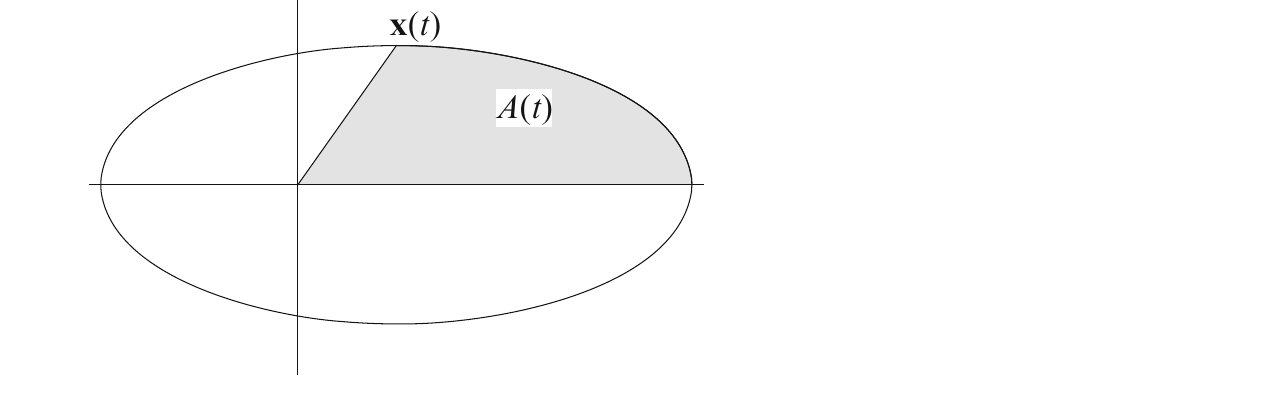
\includegraphics[width=.72\linewidth]{figures/figure-2-1.png}
  \caption{$A(t)$ 是阴影区域的面积.}\label{fig:angular-momentum-area}
\end{figure}

角动量的一个重要性质是:在某些情形下,它和能量一样是守恒的.

\begin{proposition}[旋转不变性与角动量]\label{pro:angular-momentum-conservation}
设质量为 $m$ 的粒子在 $\mathbb{R}^{2}$ 中运动,受势函数为 $V(x)$ 的保守力作用.如果 $V$ 在 $\mathbb{R}^{2}$ 的旋转下不变,那么沿牛顿方程的任意解,角动量 $J=x_{1}p_{2}-x_{2}p_{1}$ 都与时间无关.反过来,如果沿牛顿方程的每一条解,$J$ 都与时间无关,那么 $V$ 在旋转下不变.
\end{proposition}

\begin{proof}
沿一条解对式~\eqref{eq:angular-momentum-two-dimensional} 求导,得到
\begin{align*}
\frac{\mathrm{d}J}{\mathrm{d}t}
 &=\frac{\mathrm{d}x_{1}}{\mathrm{d}t}p_{2}+x_{1}\frac{\mathrm{d}p_{2}}{\mathrm{d}t}
  -\frac{\mathrm{d}x_{2}}{\mathrm{d}t}p_{1}-x_{2}\frac{\mathrm{d}p_{1}}{\mathrm{d}t}\\
 &=\frac1m p_{1}p_{2}-x_{1}\frac{\partial V}{\partial x_{2}}
  -\frac1m p_{2}p_{1}+x_{2}\frac{\partial V}{\partial x_{1}}\\
 &=x_{2}\frac{\partial V}{\partial x_{1}}-x_{1}\frac{\partial V}{\partial x_{2}}.
\end{align*}

另一方面,考虑 $\mathbb{R}^{2}$ 中的旋转 $R_{\theta}$:
\[
  R_{\theta}=\begin{pmatrix}
    \cos\theta&-\sin\theta\\
    \sin\theta&\cos\theta
  \end{pmatrix}.
\]
沿这族旋转对 $V$ 求导,可得
\[
\left.\frac{\mathrm{d}}{\mathrm{d}\theta}V(R_{\theta}x)\right|_{\theta=0}
=-x_{2}\frac{\partial V}{\partial x_{1}}+x_{1}\frac{\partial V}{\partial x_{2}}
=-\frac{\mathrm{d}J}{\mathrm{d}t}.
\]
因此,$V$ 的角向导数为零,当且仅当 $J$ 为常数.
\end{proof}

角动量的守恒结合关系式~\eqref{eq:angular-momentum-area},给出如下结果.

\begin{corollary}[Kepler 第二定律]\label{cor:kepler-second-law}
设粒子在 $\mathbb{R}^{2}$ 中运动,所受的力来自一个旋转不变的势函数.如果 $x(t)$ 是粒子的轨迹,那么在 $t=a$ 与 $t=b$ 之间,曲线 $x(t)$ 扫过的面积为
\[
  \frac{(b-a)J}{2m},
\]
其中 $J$ 是沿该轨迹恒定的角动量值.由于扫过的面积只依赖于 $b-a$,我们可以说:“相等的时间扫过相等的面积.”
\end{corollary}

当然,Kepler 研究的是在 $\mathbb{R}^{3}$ 中运动的行星,而不是 $\mathbb{R}^{2}$ 中的粒子.不过,在太阳的“平方反比”力作用下运动的行星,其运动总是位于某个平面内.(这个结论来自三维角动量守恒,见第~\ref{sec:kepler-problem} 节的说明.)

在 $\mathbb{R}^{3}$ 中,粒子的角动量是一个向量:
\begin{equation}
  J=x\times p,
  \label{eq:angular-momentum-three-dimensional}
\end{equation}
其中 $\times$ 表示叉积(或向量积).例如,
\begin{equation}
  J_{3}=x_{1}p_{2}-x_{2}p_{1}.
  \label{eq:angular-momentum-three-component}
\end{equation}
因此,如果一个 $\mathbb{R}^{3}$ 中的粒子恰好在 $\mathbb{R}^{2}$ 中运动(即 $x_{3}=0$ 且 $p_{3}=0$),那么角动量沿 $z$ 方向,其 $z$ 分量正是定义~\ref{def:angular-momentum} 中的量 $J$.

把 $\mathbb{R}^{3}$ 中粒子的角动量表示成向量,是低维空间中特有的现象.对于 $\mathbb{R}^{n}$ 中的粒子,角动量是一个斜对称矩阵:
\begin{equation}
  J_{jk}=x_{j}p_{k}-x_{k}p_{j}.
  \label{eq:angular-momentum-matrix}
\end{equation}
在 $\mathbb{R}^{3}$ 的情形,$3\times3$ 角动量矩阵的元素由角动量向量的三个分量及其负值组成,对角线上为零;可比较式~\eqref{eq:angular-momentum-three-component} 与~\eqref{eq:angular-momentum-matrix}.

\begin{definition}[系统的总角动量]\label{def:total-angular-momentum}
对于一个由 $N$ 个粒子组成、各粒子在 $\mathbb{R}^{n}$ 中运动的系统,总角动量是斜对称矩阵 $J$,其元素为
\begin{equation}
  J_{jk}=\sum_{l=1}^{N}\left(x^{l}_{j}p^{l}_{k}-x^{l}_{k}p^{l}_{j}\right).
  \label{eq:total-angular-momentum}
\end{equation}
\end{definition}

\begin{theorem}[总角动量守恒]\label{thm:total-angular-momentum}
设一个由 $N$ 个粒子组成、各粒子在 $\mathbb{R}^{n}$ 中运动的系统受到势函数为 $V$ 的保守力作用.如果对每个旋转矩阵 $R$ 都有
\begin{equation}
  V(Rx^{1},Rx^{2},\ldots,Rx^{N})=V(x^{1},x^{2},\ldots,x^{N}),
  \label{eq:rotation-invariance-many-particle}
\end{equation}
那么系统的总角动量守恒(沿每条轨迹为常数).反过来,如果总角动量沿每条轨迹都为常数,那么 $V$ 满足式~\eqref{eq:rotation-invariance-many-particle}.
\end{theorem}

这个结果的证明与命题~\ref{pro:angular-momentum-conservation} 的证明类似,留作练习(练习 10).下一节中,我们将用 Poisson 括号和 Hamilton 流的语言重新考察角动量的概念.

\section{Poisson 括号与 Hamilton 力学}

现在考虑经典力学的 Hamilton 处理方式.(此外还有 Lagrange 处理方式,但它与我们的目的不太相关.)Hamilton 处理方式,尤其是 Poisson 括号,将帮助我们理解守恒量的一般现象.Poisson 括号也是量子力学中使用对易子的一个重要动机来源.

在 Hamilton 处理方式中,我们把能量函数看成位置和动量的函数,而不是位置和速度的函数,并把它称为“Hamilton 函数”.如果 $\mathbb{R}^{n}$ 中的粒子具有通常的能量函数(动能加势能),则
\begin{equation}
  H(x,p)=\frac{1}{2m}\sum_{j=1}^{n}p_{j}^{2}+V(x).
  \label{eq:hamiltonian-one-particle}
\end{equation}
这里和通常一样,$p_{j}=m\dot{x}_{j}$.现在注意,牛顿定律可以写成
\begin{equation}
  \frac{\mathrm{d}x_{j}}{\mathrm{d}t}=\frac{\partial H}{\partial p_{j}},
  \qquad
  \frac{\mathrm{d}p_{j}}{\mathrm{d}t}=-\frac{\partial H}{\partial x_{j}}.
  \label{eq:hamilton-equations}
\end{equation}
事实上,对于形式~\eqref{eq:hamiltonian-one-particle} 的 $H$,这些方程给出 $\mathrm{d}x_{j}/\mathrm{d}t=p_{j}/m$,这正是 $p_{j}$ 的定义;同时 $\mathrm{d}p_{j}/\mathrm{d}t=-\partial V/\partial x_{j}=F_{j}$,这正是最初形式的牛顿定律.我们把形式~\eqref{eq:hamilton-equations} 的牛顿定律称为 Hamilton 方程.

虽然目前还不明显,把牛顿定律写成式~\eqref{eq:hamilton-equations} 的形式究竟带来了什么好处,但我们继续往下看.下一步是引入 Poisson 括号.

\begin{definition}[Poisson 括号]\label{def:poisson-bracket}
设 $f$ 和 $g$ 是 $\mathbb{R}^{2n}$ 上的两个光滑函数.把 $\mathbb{R}^{2n}$ 中的元素看成一对 $(x,p)$,其中 $x\in\mathbb{R}^{n}$ 表示粒子的位置,$p\in\mathbb{R}^{n}$ 表示粒子的动量.$f$ 与 $g$ 的 Poisson 括号记为 $\{f,g\}$,是 $\mathbb{R}^{2n}$ 上的函数,定义为
\begin{equation}
  \{f,g\}(x,p)=\sum_{j=1}^{n}\left(\frac{\partial f}{\partial x_{j}}\frac{\partial g}{\partial p_{j}}-\frac{\partial f}{\partial p_{j}}\frac{\partial g}{\partial x_{j}}\right).
  \label{eq:poisson-bracket}
\end{equation}
\end{definition}

Poisson 括号具有下列性质.

\begin{proposition}[Poisson 括号的性质]\label{pro:poisson-properties}
对 $\mathbb{R}^{2n}$ 上的任意光滑函数 $f,g,h$,有:
\begin{enumerate}
  \item 对任意 $c\in\mathbb{R}$,$\{f,g+ch\}=\{f,g\}+c\{f,h\}$;
  \item $\{g,f\}=-\{f,g\}$;
  \item $\{f,gh\}=\{f,g\}h+g\{f,h\}$;
  \item $\{f,\{g,h\}\}=\{\{f,g\},h\}+\{g,\{f,h\}\}$.
\end{enumerate}
\end{proposition}

命题~\ref{pro:poisson-properties} 的前两条性质说明 Poisson 括号是双线性的并且斜对称.第三条性质说明,“与 $f$ 作括号”这一运算相对于函数的逐点乘法满足导子性质(类似于导数的乘积法则);第四条性质则说明,“与 $f$ 作括号”相对于 Poisson 括号本身也满足导子性质.第四条性质等价于 Jacobi 恒等式
\begin{equation}
  \{f,\{g,h\}\}+\{h,\{f,g\}\}+\{g,\{h,f\}\}=0.
  \label{eq:poisson-jacobi}
\end{equation}
这可以利用 Poisson 括号的斜对称性直接验证.Jacobi 恒等式与双线性、斜对称性一起说明,$\mathbb{R}^{2n}$ 上的 $C^{\infty}$ 函数空间在 Poisson 括号运算下构成一个李代数(见第 16 章).

\begin{proof}
Poisson 括号的前两条性质显然成立,第三条是乘积法则的直接结果.我们说明如何直接计算第四条性质.(练习 15 给出了另一种证明.)计算可得
\[
\{f,\{g,h\}\}
=\sum_{j=1}^{n}\left[
\frac{\partial f}{\partial x_{j}}\frac{\partial}{\partial p_{j}}
  \left(\frac{\partial g}{\partial x_{j}}\frac{\partial h}{\partial p_{j}}-\frac{\partial g}{\partial p_{j}}\frac{\partial h}{\partial x_{j}}\right)
-\frac{\partial f}{\partial p_{j}}\frac{\partial}{\partial x_{j}}
  \left(\frac{\partial g}{\partial x_{j}}\frac{\partial h}{\partial p_{j}}-\frac{\partial g}{\partial p_{j}}\frac{\partial h}{\partial x_{j}}\right)
\right].
\]
例如,第一项使用乘积法则后会产生四项(这里及下文都对 $j$ 求和):
\begin{align}
&\frac{\partial f}{\partial x_{j}}\frac{\partial^{2}g}{\partial x_{j}\partial p_{j}}\frac{\partial h}{\partial p_{j}}
 +\frac{\partial f}{\partial x_{j}}\frac{\partial g}{\partial x_{j}}\frac{\partial^{2}h}{\partial p_{j}^{2}}
 -\frac{\partial f}{\partial x_{j}}\frac{\partial^{2}g}{\partial p_{j}^{2}}\frac{\partial h}{\partial x_{j}}
 -\frac{\partial f}{\partial x_{j}}\frac{\partial g}{\partial p_{j}}\frac{\partial^{2}h}{\partial x_{j}\partial p_{j}}.
\label{eq:poisson-proof-four-terms}
\end{align}
因此,式~\eqref{eq:poisson-jacobi} 左边总共有 24 项,每一项都对 $j$ 求和.每一项在三个函数中的两个函数上各有一个导数,在第三个函数上有两个导数.两阶导数落在哪个函数上共有三种可能;选定该函数后,另外两个函数上的导数有四种分配方式,而承担二阶导数的函数上的导数也随之确定(总共需要两个 $x$ 导数和两个 $p$ 导数).所以共有 12 种可能的项.直接而繁琐的检查表明,这 12 种项中的每一项都会在式~\eqref{eq:poisson-jacobi} 的左边出现两次,且符号相反.例如,在计算 $\{h,\{f,g\}\}$ 时,会得到一个与式~\eqref{eq:poisson-proof-four-terms} 的第二项类似的项,只需把 $(f,g,h)$ 换成 $(h,f,g)$:
\[
  \frac{\partial h}{\partial x_{j}}\frac{\partial f}{\partial x_{j}}\frac{\partial^{2}g}{\partial p_{j}^{2}}.
\]
这一项(出现在计算 $\{h,\{f,g\}\}$ 的过程中)恰好与式~\eqref{eq:poisson-proof-four-terms} 的第三项抵消(后者出现在计算 $\{f,\{g,h\}\}$ 的过程中).
\end{proof}

下面的初等结果将为量子力学中的“正则对易关系”提供有用的类比.

\begin{proposition}[位置与动量的 Poisson 括号]\label{pro:canonical-poisson-relations}
位置函数与动量函数满足
\[
  \{x_{j},x_{k}\}=0,\qquad
  \{p_{j},p_{k}\}=0,\qquad
  \{x_{j},p_{k}\}=\delta_{jk}.
\]
\end{proposition}

\begin{proof}
直接计算即可.
\end{proof}

考虑 Poisson 括号的另一个主要原因,是下面这个简单结果.

\begin{proposition}[沿 Hamilton 轨道的导数]\label{pro:derivative-poisson}
如果 $(x(t),p(t))$ 是 Hamilton 方程~\eqref{eq:hamilton-equations} 的一个解,那么对 $\mathbb{R}^{2n}$ 上任意光滑函数 $f$,都有
\begin{equation}
  \frac{\mathrm{d}}{\mathrm{d}t}f(x(t),p(t))=\{f,H\}(x(t),p(t)).
  \label{eq:derivative-poisson}
\end{equation}
\end{proposition}

通常把命题~\ref{pro:derivative-poisson} 更简洁地写成
\[
  \frac{\mathrm{d}f}{\mathrm{d}t}=\{f,H\},
\]
其中时间导数理解为沿某条轨迹的导数.

\begin{proof}
利用链式法则和 Hamilton 方程,
\begin{align*}
\frac{\mathrm{d}f}{\mathrm{d}t}
 &=\sum_{j=1}^{n}\left(\frac{\partial f}{\partial x_{j}}\frac{\mathrm{d}x_{j}}{\mathrm{d}t}+\frac{\partial f}{\partial p_{j}}\frac{\mathrm{d}p_{j}}{\mathrm{d}t}\right)\\
 &=\sum_{j=1}^{n}\left(\frac{\partial f}{\partial x_{j}}\frac{\partial H}{\partial p_{j}}-\frac{\partial f}{\partial p_{j}}\frac{\partial H}{\partial x_{j}}\right)\\
 &=\{f,H\},
\end{align*}
这正是所要证明的结论.
\end{proof}

注意,取 $f(x,p)=x_{j}$ 或 $f(x,p)=p_{j}$,命题~\ref{pro:derivative-poisson} 就包含了 Hamilton 方程本身.因此,这个命题给出了表达时间演化的一种与坐标无关的方式.

\begin{corollary}[守恒量与 Poisson 括号]\label{cor:poisson-conserved-quantity}
称 $\mathbb{R}^{2n}$ 上的光滑函数 $f$ 是一个守恒量,如果对 Hamilton 方程的每条解 $(x(t),p(t))$,$f(x(t),p(t))$ 都与 $t$ 无关.那么 $f$ 是守恒量,当且仅当
\[
  \{f,H\}=0.
\]
特别地,Hamilton 函数 $H$ 是守恒量.
\end{corollary}

守恒量也称为运动常数.关于这个结果的另一种观点,见结论 2.31.守恒量(如果能够找到)很有用,因为我们知道轨迹必须位于每个守恒量的等值面内.例如,设粒子在 $\mathbb{R}^{2}$ 中运动,Hamilton 函数 $H$ 和另一个独立函数 $f$(比如角动量)都是守恒量.那么我们不必在四维相空间中寻找轨迹,而只需在 $H$ 和 $f$ 的联合等值集内寻找轨迹,即寻找形如 $H(x,p)=a$、$f(x,p)=b$(其中 $a,b$ 是常数)的集合.这些联合等值集通常是二维的,而不是四维的,因此守恒量把问题从四个变量的方程大幅简化成了两个变量的方程.

在 $\mathbb{R}^{2n}$ 上求解 Hamilton 方程,会产生一个流,即一族 $\mathbb{R}^{2n}$ 的微分同胚 $\Phi_{t}$;其中 $\Phi_{t}(x,p)$ 等于以 $(x,p)$ 为初始条件的 Hamilton 方程在时间 $t$ 的解.根据势函数 $V$ 的选择,粒子可能在有限时间内逃到无穷远,因此映射 $\Phi_{t}$ 不一定在整个 $\mathbb{R}^{2n}$ 上有定义,而可能只在其中某个开子集上有定义.如果 $\Phi_{t}$ 对所有 $t$ 都在整个 $\mathbb{R}^{2n}$ 上有定义,我们就称这个流是\emph{完备的}.

\begin{theorem}[Liouville 定理]\label{thm:liouville}
任意 Hamilton 函数 $H$ 的 Hamilton 方程所对应的流,都保持 $(2n)$ 维体积测度
\[
  \mathrm{d}x_{1}\,\mathrm{d}x_{2}\cdots\mathrm{d}x_{n}\,\mathrm{d}p_{1}\,\mathrm{d}p_{2}\cdots\mathrm{d}p_{n}
\]
不变.

更准确地说,如果可测集 $E$ 对某个 $t\in\mathbb{R}$ 包含在 $\Phi_{t}$ 的定义域中,那么 $\Phi_{t}(E)$ 的体积等于 $E$ 的体积.
\end{theorem}

\begin{proof}
Hamilton 方程可以写成
\begin{equation}
\frac{\mathrm{d}}{\mathrm{d}t}
\begin{pmatrix}
 x_{1}\\ \vdots\\ x_{n}\\ p_{1}\\ \vdots\\ p_{n}
\end{pmatrix}
=
\begin{pmatrix}
 \partial H/\partial p_{1}\\ \vdots\\ \partial H/\partial p_{n}\\
 -\partial H/\partial x_{1}\\ \vdots\\ -\partial H/\partial x_{n}
\end{pmatrix}.
\label{eq:hamilton-vector-field}
\end{equation}
这意味着 Hamilton 方程描述了 $\mathbb{R}^{2n}$ 上沿式~\eqref{eq:hamilton-vector-field} 右端向量场的流.向量分析的一个标准结果(例如见 [29] 中的命题 16.33)表明,当且仅当该向量场的散度为零时,这个流保持体积.我们计算散度得到
\[
  \frac{\partial}{\partial x_{1}}\frac{\partial H}{\partial p_{1}}+\cdots+\frac{\partial}{\partial x_{n}}\frac{\partial H}{\partial p_{n}}
  -\frac{\partial}{\partial p_{1}}\frac{\partial H}{\partial x_{1}}-\cdots-\frac{\partial}{\partial p_{n}}\frac{\partial H}{\partial x_{n}}.
\]
由于
\[
  \frac{\partial^{2}H}{\partial x_{j}\partial p_{j}}
  =\frac{\partial^{2}H}{\partial p_{j}\partial x_{j}},
\]
所以散度为零.
\end{proof}

不变体积的存在对系统动力学有重要后果.例如,对于“受限”系统,不变体积意味着系统表现出“回归性”:粗略地说,对大多数初始条件,粒子最终都会在相空间中任意接近其初始状态.不过,我们不在这里深入讨论这一点.

注意,式~\eqref{eq:hamilton-vector-field} 中计算出的 $X_{H}$ 的散度以一种非常特殊的方式为零,即第 $j$ 项与第 $(n+j)$ 项对每个 $1\leq j\leq n$ 都分别抵消.事实证明,这个更强的条件等价于:任意 $\mathbb{R}^{2n}$ 上的光滑函数所对应的 Hamilton 流 $\Phi_{t}$ 保持辛形式 $\omega$ 不变,其中
\[
  \omega\bigl((x,p),(x',p')\bigr)=x\cdot p'-p\cdot x'.
\]
更准确地说,对任意 $t\in\mathbb{R}$ 和任意 $(x,p)\in\mathbb{R}^{2n}$,把 $\Phi_{t}$ 在 $(x,p)$ 处的偏导数矩阵看成从 $\mathbb{R}^{2n}$ 到 $\mathbb{R}^{2n}$ 的线性映射,它保持 $\omega$ 不变.事实证明,$\Phi_{t}$ 的这一性质等价于它保持 Poisson 括号,即对所有 $f,g\in C^{\infty}(\mathbb{R}^{n})$,
\[
  \{f\circ\Phi_{t},g\circ\Phi_{t}\}=\{f,g\}\circ\Phi_{t}.
\]
保持 $\omega$ 的映射 $\Psi:\mathbb{R}^{2n}\to\mathbb{R}^{2n}$ 在数学记号中称为辛同胚,在物理学记号中称为正则变换.我们把这些结论的证明推迟到第 21 章,到那时我们将在更一般的情形下讨论它们.

\begin{definition}[Hamilton 流的生成元]\label{def:hamiltonian-generator}
对 $\mathbb{R}^{2n}$ 上的任意光滑函数 $f$,把 Hamilton 方程~\eqref{eq:hamilton-equations} 中的 Hamilton 函数 $H$ 换成 $f$,求解所得的流称为由 $f$ 生成的 Hamilton 流;函数 $f$ 称为相应流的 Hamilton 生成元.
\end{definition}

虽然任意光滑函数都可以代入 Hamilton 方程以产生一个流,但从物理上看,应当认为系统有一个特殊的函数,即系统的 Hamilton 函数 $H$,由 $H$ 生成的流才是系统的时间演化.对于其他函数 $f$,由 $f$ 生成的 Hamilton 流不应被理解为时间演化,而应理解为某种其他的流,例如它可能表示系统的一族对称性.

\begin{proposition}[平移的 Hamilton 流]\label{pro:hamiltonian-translations}
函数
\begin{equation}
  f_{a}(x,p):=a\cdot p
  \label{eq:hamiltonian-position-translation}
\end{equation}
生成的 Hamilton 流为
\begin{equation}
  x(t)=x_{0}+ta,\qquad p(t)=p_{0}.
  \label{eq:hamiltonian-position-translation-flow}
\end{equation}
函数
\begin{equation}
  g_{b}(x,p):=b\cdot x
  \label{eq:hamiltonian-momentum-translation}
\end{equation}
生成的 Hamilton 流为
\[
  x(t)=x_{0},\qquad p(t)=p_{0}-tb.
\]
\end{proposition}

\begin{proof}
直接计算即可.
\end{proof}

这意味着,由动量函数的线性组合生成的 Hamilton 流,是对粒子位置作平移.也就是说,在式~\eqref{eq:hamiltonian-position-translation} 中由 $f_{a}$ 生成的流~\eqref{eq:hamiltonian-position-translation-flow} 中,粒子的初始位置 $x_{0}$ 被平移了 $ta$,而粒子的动量与 $t$ 无关.同样地,由位置函数的线性组合(函数 $g_{b}$)生成的 Hamilton 流,是对粒子动量作平移.

\begin{proposition}[角动量生成旋转]\label{pro:angular-momentum-flow}
对一个在 $\mathbb{R}^{2}$ 中运动的粒子,角动量函数
\[
  J(x,p)=x_{1}p_{2}-x_{2}p_{1}
\]
所生成的 Hamilton 流由 $x$ 和 $p$ 的同时旋转组成,即
\begin{equation}
  \begin{pmatrix}x_{1}(t)\\x_{2}(t)\end{pmatrix}
  =\begin{pmatrix}\cos t&-\sin t\\\sin t&\cos t\end{pmatrix}
   \begin{pmatrix}x_{1}(0)\\x_{2}(0)\end{pmatrix},
  \qquad
  \begin{pmatrix}p_{1}(t)\\p_{2}(t)\end{pmatrix}
  =\begin{pmatrix}\cos t&-\sin t\\\sin t&\cos t\end{pmatrix}
   \begin{pmatrix}p_{1}(0)\\p_{2}(0)\end{pmatrix}.
  \label{eq:angular-momentum-hamiltonian-flow}
\end{equation}
\end{proposition}

\begin{proof}
将角动量函数 $J$ 代替 Hamilton 方程中的 $H$,得到
\[
  \frac{\mathrm{d}x_{1}}{\mathrm{d}t}=\frac{\partial J}{\partial p_{1}}=-x_{2},
  \qquad
  \frac{\mathrm{d}p_{1}}{\mathrm{d}t}=-\frac{\partial J}{\partial x_{1}}=-p_{2},
\]
\[
  \frac{\mathrm{d}x_{2}}{\mathrm{d}t}=\frac{\partial J}{\partial p_{2}}=x_{1},
  \qquad
  \frac{\mathrm{d}p_{2}}{\mathrm{d}t}=-\frac{\partial J}{\partial x_{2}}=p_{1}.
\]
这个系统的解由式~\eqref{eq:angular-momentum-hamiltonian-flow} 给出,直接求导即可验证.
\end{proof}

注意,由 $J$ 生成的 Hamilton 流并不具有粒子时间演化的解释,所以式~\eqref{eq:angular-momentum-hamiltonian-flow} 中的参数 $t$ 不应解释为物理时间;它只是一个一参数微分同胚群中的参数.在这里,$t$ 是旋转角.因此,对“角动量是什么？”这个问题,一个答案是:$J$ 是旋转的 Hamilton 生成元.

如果 $f$ 是任意光滑函数,那么根据命题~\ref{pro:derivative-poisson} 的证明,沿由 $f$ 生成的 Hamilton 流,另一个函数 $g$ 的时间导数为 $\mathrm{d}g/\mathrm{d}t=\{g,f\}$.特别地,Hamilton 函数 $H$ 沿由 $f$ 生成的流的导数是 $\{H,f\}$.因此,$f$ 沿由 $H$ 生成的流为常数,当且仅当 $\{f,H\}=0$;这又当且仅当 $H$ 沿由 $f$ 生成的流为常数.这个推理给出如下结论.

\begin{conclusion}
函数 $f$ 对 Hamilton 方程~\eqref{eq:hamilton-equations} 的解来说是守恒量,当且仅当 $H$ 在由 $f$ 生成的 Hamilton 流下不变.特别地,角动量 $J$ 守恒,当且仅当 $H$ 在 $x$ 和 $p$ 的同时旋转下不变.
\end{conclusion}

我们将在第 21 章回到这种理解守恒量的方式.另见练习 12.

Hamilton 框架可以直接推广到粒子系统.

\begin{proposition}[多粒子 Hamilton 系统]\label{pro:many-particle-hamiltonian}
考虑一个由 $N$ 个粒子组成、各粒子在 $\mathbb{R}^{n}$ 中运动的系统,其相空间为 $\mathbb{R}^{2nN}$,可以看成形如
\[
  (x^{1},\ldots,x^{N},p^{1},\ldots,p^{N})
\]
的 $(2N)$ 元组所成的集合,其中 $x^{j},p^{j}\in\mathbb{R}^{n}$.在相空间上,对两个光滑函数 $f,g$ 定义 Poisson 括号
\[
  \{f,g\}=\sum_{j=1}^{N}\sum_{k=1}^{n}\left(
  \frac{\partial f}{\partial x^{j}_{k}}\frac{\partial g}{\partial p^{j}_{k}}
  -\frac{\partial f}{\partial p^{j}_{k}}\frac{\partial g}{\partial x^{j}_{k}}\right),
\]
并考虑形式为
\[
  H(x^{1},\ldots,x^{N},p^{1},\ldots,p^{N})
  =\sum_{j=1}^{N}\frac{1}{2m_{j}}\lvert p^{j}\rvert^{2}+V(x^{1},\ldots,x^{N})
\]
的 Hamilton 函数.那么,形式为 $m_{j}\ddot{x}^{j}=-\nabla_{j}V$ 的牛顿定律等价于 Hamilton 方程
\begin{equation}
  \frac{\mathrm{d}x^{j}_{k}}{\mathrm{d}t}=\frac{\partial H}{\partial p^{j}_{k}},
  \qquad
  \frac{\mathrm{d}p^{j}_{k}}{\mathrm{d}t}=-\frac{\partial H}{\partial x^{j}_{k}}.
  \label{eq:many-particle-hamilton-equations}
\end{equation}
对 Hamilton 方程的任意解和任意光滑函数 $f$,都有
\[
  \frac{\mathrm{d}f}{\mathrm{d}t}=\{f,H\}.
\]
\end{proposition}

这个结果的证明与单粒子情形完全类似,故略去.

\section{Kepler 问题与 Runge--Lenz 向量}\label{sec:kepler-problem}

\subsection{Kepler 问题}\label{subsec:kepler-problem}

现在考虑经典的 Kepler 问题,即寻找行星绕太阳运动的轨迹.由于太阳的质量远大于任何一颗行星,我们可以把太阳的位置看成固定在坐标系原点.太阳对行星施加的力为
\begin{equation}
  F=-k\frac{x}{\lvert x\rvert^{3}},
  \label{eq:kepler-force}
\end{equation}
其中 $k=GmM$,$m$ 是行星质量,$M$ 是太阳质量,$G$ 是万有引力常数.注意,$F$ 的大小与到原点距离的平方的倒数成正比,因此这个力满足平方反比定律.由于 $k$ 含有行星质量 $m$ 这一因子,而运动方程是 $m\ddot{x}=F$,所以 $m$ 会从运动方程中约掉.与力~\eqref{eq:kepler-force} 对应的势能显然是
\begin{equation}
  V(x)=-\frac{k}{\lvert x\rvert}.
  \label{eq:kepler-potential}
\end{equation}

由于势能 $V$ 在旋转下不变,角动量向量 $J=x\times p$ 是守恒量(定理~\ref{thm:total-angular-momentum},取 $N=1$、$n=3$).如果 $J=0$,粒子沿着经过原点的一条射线运动.在这种情况下,如果初始动量指向原点,粒子将在未来某时刻穿过原点;如果初始动量背离原点,则粒子必定在过去某时刻穿过原点.这类轨迹称为\emph{碰撞轨迹},我们将把它们视为病态情形.

从现在开始,我们只考虑角动量向量非零的轨迹.固定粒子的能量和角动量,会保证粒子始终与原点保持某个最小距离(见练习 20).另一方面,由于 $J=x\times p$,粒子的位置 $x(t)$ 始终垂直于 $J$ 的恒定值.因此,我们把经过原点且垂直于 $J$ 的平面称为\emph{运动平面}.

\subsection{Runge--Lenz 向量的守恒}

我们将借助一个称为 Runge--Lenz 向量的对象,以间接方式描述经典轨迹.

\begin{definition}[Runge--Lenz 向量]\label{def:runge-lenz-vector}
Runge--Lenz 向量是在 $(\mathbb{R}^{3}\setminus\{0\})\times\mathbb{R}^{3}$ 上取向量值的函数,定义为
\begin{equation}
  A(x,p)=\frac{1}{mk}\,p\times J-\frac{x}{\lvert x\rvert}.
  \label{eq:runge-lenz-vector}
\end{equation}
这里 $x$ 表示经典粒子的位置,$p$ 表示其动量.
\end{definition}

这个向量的重要性在于:对于 Kepler 问题,它是一个守恒量.当然,只要势能是径向的(即距离原点的函数),角动量向量就是守恒量.Kepler 问题中形如 $1/r$ 的势能之所以特殊,是因为它还有另一个守恒的向量值量.

\begin{proposition}[Runge--Lenz 向量守恒]\label{pro:runge-lenz-conservation}
对受力~\eqref{eq:kepler-force} 作用而满足 Newton 定律的粒子,Runge--Lenz 向量是守恒量.
\end{proposition}

\begin{proof}
由于 $J$ 守恒,我们计算得到
\begin{align*}
\dot{A}(t)
 &=\frac{1}{mk}F\times J-\frac{1}{m}\frac{\mathrm{d}}{\mathrm{d}t}\left(\frac{x}{\lvert x\rvert}\right)\\
 &=-\frac{1}{m\lvert x\rvert^{3}}x\times(x\times p)-\frac{1}{m}\left(\frac{p}{\lvert x\rvert}-\frac{x(x\cdot p)}{\lvert x\rvert^{3}}\right)\\
 &=\frac1m\left[-\frac{x(x\cdot p)}{\lvert x\rvert^{3}}+\frac{p(x\cdot x)}{\lvert x\rvert^{3}}-\frac{p}{\lvert x\rvert}+\frac{x(x\cdot p)}{\lvert x\rvert^{3}}\right]\\
 &=0.
\end{align*}
这里使用了对所有 $b,c,d\in\mathbb{R}^{3}$ 都成立的恒等式
\[
  b\times(c\times d)=c(b\cdot d)-d(b\cdot c).
\]
\end{proof}

\subsection{椭圆、双曲线和抛物线}

现在利用 Runge--Lenz 向量确定 Kepler 问题的轨迹.

\begin{proposition}[Runge--Lenz 向量的大小]\label{pro:runge-lenz-magnitude}
Runge--Lenz 向量 $A$ 的大小满足
\begin{equation}
  \lvert A\rvert^{2}=1+\frac{2\lvert J\rvert^{2}}{mk^{2}}E,
  \label{eq:runge-lenz-magnitude}
\end{equation}
其中 $E=\lvert p\rvert^{2}/(2m)-k/\lvert x\rvert$ 是粒子的能量.此外,如果 $\widehat{x}:=x/\lvert x\rvert$ 是 $x$ 方向上的单位向量,那么对所有非零 $x$ 都有
\begin{equation}
  A\cdot\widehat{x}=\frac{\lvert J\rvert^{2}}{mk\lvert x\rvert}-1.
  \label{eq:runge-lenz-radial-relation}
\end{equation}
由此得到
\begin{equation}
  \lvert x\rvert=\frac{\lvert J\rvert^{2}}{mk(1+A\cdot\widehat{x})}.
  \label{eq:kepler-radial-equation}
\end{equation}
注意,从式~\eqref{eq:runge-lenz-radial-relation} 可知,对所有 $x\neq0$,都有 $A\cdot\widehat{x}>-1$.
\end{proposition}

\begin{proof}
利用恒等式 $b\cdot(c\times d)=d\cdot(b\times c)$,可得
\[
  \widehat{x}\cdot(p\times J)=J\cdot(\widehat{x}\times p)=\frac{\lvert J\rvert^{2}}{\lvert x\rvert}.
\]
由于 $J$ 与 $p$ 正交,
\begin{align*}
\lvert A\rvert^{2}
 &=\frac{1}{m^{2}k^{2}}\lvert p\rvert^{2}\lvert J\rvert^{2}+1-\frac{2}{mk}\widehat{x}\cdot(p\times J)\\
 &=1+\frac{2\lvert J\rvert^{2}}{mk}\left(\frac{\lvert p\rvert^{2}}{2m}-\frac{k}{\lvert x\rvert}\right)\\
 &=1+\frac{2\lvert J\rvert^{2}}{mk^{2}}E.
\end{align*}
再次使用 $b\cdot(c\times d)=d\cdot(b\times c)$,得到
\[
  A\cdot x=\frac{1}{mk}J\cdot(x\times p)-\frac{x\cdot x}{\lvert x\rvert}
  =\frac{\lvert J\rvert^{2}}{mk}-\lvert x\rvert.
\]
两边除以 $\lvert x\rvert$,便得到 $A\cdot\widehat{x}$ 的表达式;再解出 $\lvert x\rvert$ 即得结论.
\end{proof}

\begin{corollary}[Kepler 轨道的极坐标方程]\label{cor:kepler-polar-equation}
在运动平面内选取一组正交坐标,使 $A$ 沿正 $x_{1}$ 轴方向.若 $(r,\theta)$ 是与这组坐标对应的极坐标,那么沿每条轨迹 $(r(t),\theta(t))$ 都有
\begin{equation}
  r(t)=\frac{\lvert J\rvert^{2}}{mk\bigl(1+A\cos\theta(t)\bigr)},
  \label{eq:kepler-polar-orbit}
\end{equation}
其中 $A=\lvert A\rvert$.如果 $A=0$,则可以使用任意正交坐标.
\end{corollary}

\begin{proposition}[Kepler 轨道的类型]\label{pro:kepler-orbit-types}
如果 $A:=\lvert A\rvert<1$,则式~\eqref{eq:kepler-polar-orbit} 是一条离心率为 $A$、且原点为其一个焦点的椭圆方程.如果 $A>1$,它是双曲线方程;如果 $A=1$,它是抛物线方程.

粒子在运动平面内的轨道,在粒子能量为负时是椭圆,在能量为正时是双曲线,在能量为零时是抛物线.
\end{proposition}

\begin{figure}[htbp]
  \centering
  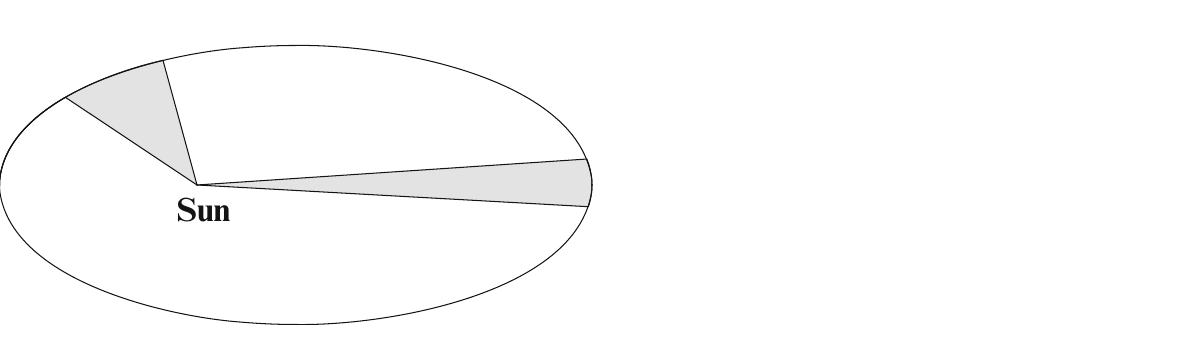
\includegraphics[width=.70\linewidth]{figures/figure-2-2.png}
  \caption{Kepler 问题中的椭圆轨道,阴影部分为两个相等的面积.}\label{fig:kepler-ellipse}
\end{figure}

Kepler 第一定律断言,行星沿椭圆轨道运动,太阳位于其中一个焦点,如图~\ref{fig:kepler-ellipse} 所示.阴影区域表示在相等时间内扫过的两个相等面积,这与 Kepler 第二定律(推论~\ref{cor:kepler-second-law})一致.

回忆一下,椭圆的离心率为 $\sqrt{1-(b/a)^{2}}$,其中 $a$ 是长轴长度的一半,$b$ 是短轴长度的一半.因此,当 $A=0$ 时,$b=a$,椭圆就是圆.

\begin{proof}
继续在 $A$ 沿正 $x_{1}$ 轴方向的坐标系中工作.此时式~\eqref{eq:kepler-polar-orbit} 变为
\[
  \sqrt{x^{2}+y^{2}}=\alpha\frac{1}{1+A\dfrac{x}{\sqrt{x^{2}+y^{2}}}},
\]
其中 $\alpha=\lvert J\rvert^{2}/(mk)$.由此得到
\[
  1=\frac1\alpha\left(\sqrt{x^{2}+y^{2}}+Ax\right).
\]
现在解出 $\sqrt{x^{2}+y^{2}}$,将方程两边平方并化简.假设 $A^{2}\neq1$,可得
\begin{equation}
  \alpha^{2}\left(\frac{1}{1-A^{2}}\right)
  =(1-A^{2})\left(x+\frac{A\alpha}{1-A^{2}}\right)^{2}+y^{2}.
  \label{eq:kepler-conic-equation}
\end{equation}
这是椭圆(若 $A^{2}<1$)或双曲线(若 $A^{2}>1$)的方程,其中心为 $(-\alpha/(1-A^{2}),0)$.结合命题~\ref{pro:runge-lenz-magnitude} 中关于 $A:=\lvert A\rvert$ 的公式,可知粒子能量为负时得到椭圆,能量为正时得到双曲线.

当 $A^{2}<1$ 时,可以直接计算出椭圆长轴和短轴的半长分别为
\[
  a=\frac{\alpha}{1-A^{2}},
  \qquad
  b=\frac{\alpha}{\sqrt{1-A^{2}}}.
\]
由此容易算出离心率为 $A$.椭圆两焦点之间的距离等于长轴长度乘以离心率,在这里为 $2A\alpha/(1-A^{2})$.由于式~\eqref{eq:kepler-conic-equation} 中椭圆的中心是 $( -A\alpha/(1-A^{2}),0)$,原点正好是椭圆的一个焦点.

如果 $A^{2}=1$,进行同样的分析时,$x^{2}$ 项会从方程中消失,得到
\[
  x=\frac{1}{2A\alpha}\left(-y^{2}+\alpha^{2}\right),
\]
这是沿 $x$ 轴开口的抛物线方程.这种情形对应于能量为零.
\end{proof}

注意,命题~\ref{pro:kepler-orbit-types} 没有告诉我们粒子作为时间函数如何沿椭圆、双曲线或抛物线运动.不过,原则上可以利用角动量确定这一点.事实上,在运动平面中应用式~\eqref{eq:angular-momentum-polar},得到
\begin{equation}
  \frac{\mathrm{d}\theta}{\mathrm{d}t}=\frac{1}{mr^{2}}\lvert J\rvert,
  \label{eq:kepler-angular-speed}
\end{equation}
其中 $\theta$ 是运动平面内的极角变量.由于推论~\ref{cor:kepler-polar-equation} 已经给出了 $r$ 关于 $\theta$ 的函数关系,式~\eqref{eq:kepler-angular-speed} 给出一个(一阶、可分离变量的)微分方程;我们可以尝试求解它,从而得到 $\theta$——以及 $r$——关于 $t$ 的函数.

\subsection{Kepler 问题的特殊性质}

如前所述,除了守恒的能量和角动量之外,还存在另一个守恒的向量值函数,这是势能取 $-k/\lvert x\rvert$ 形式所特有的.对于一般的径向势能,能量和角动量将是仅有的守恒量.假设 $J\neq0$,任意径向势能中的粒子运动总是位于垂直于 $J$ 的平面内.考虑到这一点,我们可以把粒子看成在 $\mathbb{R}^{2}$ 而不是 $\mathbb{R}^{3}$ 中运动,并相应地把相空间看成四维而不是六维.从这个角度看,还剩下两个守恒量,即能量 $E$ 和运动平面中的标量角动量 $J$(如定义~\ref{def:angular-momentum} 所给出).因此,每条轨迹都位于形如
\[
  \left\{(x,p)\in\mathbb{R}^{2}\times\mathbb{R}^{2}:E(x,p)=a,\ J(x,p)=b\right\}
\]
的集合中.这种集合称为 $E$ 与 $J$ 的\emph{联合等值集}.这些集合是四维相空间中的二维曲面.

对于一般的径向势能,相空间中的轨迹 $(x(t),p(t))$ 可能不是一条闭曲线,而是在它所在的联合等值面中填满一个稠密子集.特别地,位置空间中的轨迹 $x(t)$ 通常不是闭曲线.例如,$x(t)$ 可能在运动平面内描出一个大致椭圆形的区域,但椭圆的轴会发生“进动”,也就是随时间变化.图~\ref{fig:radial-potential-precession} 展示了这样一条轨迹;应将它与图~\ref{fig:kepler-ellipse} 对照.

\begin{figure}[htbp]
  \centering
  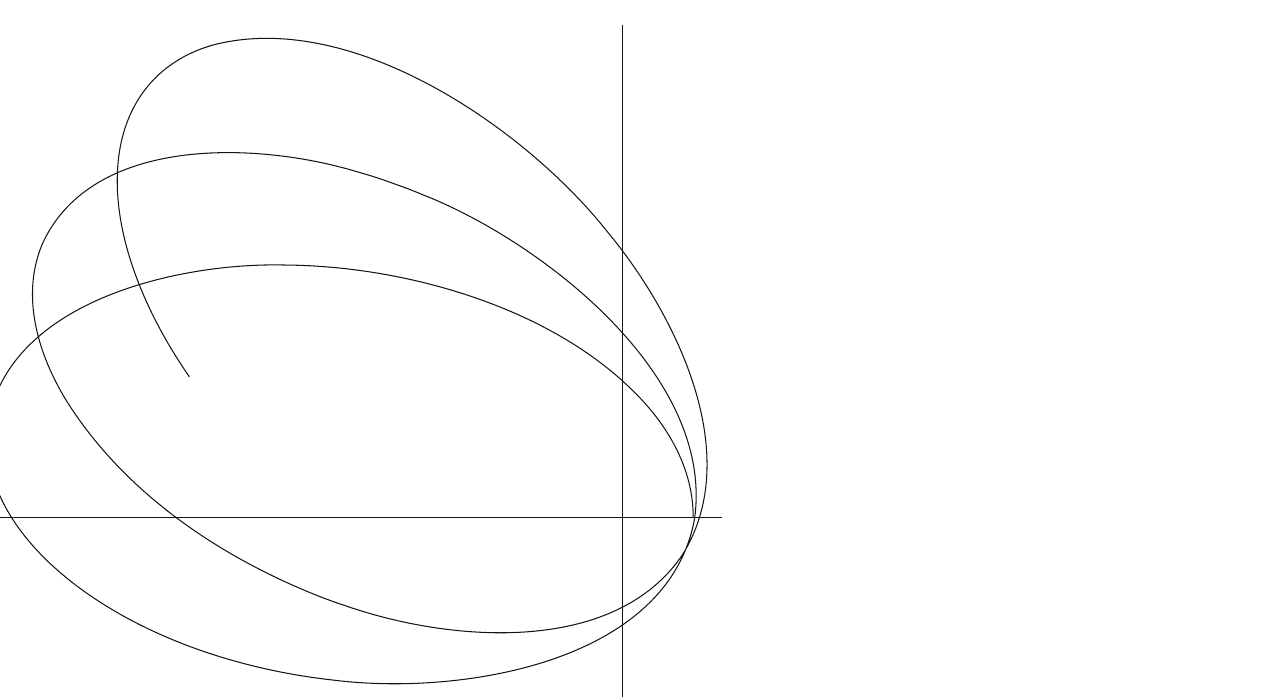
\includegraphics[width=.70\linewidth]{figures/figure-2-3.png}
  \caption{典型径向势能下,运动平面内的轨迹.}\label{fig:radial-potential-precession}
\end{figure}

在 Kepler 问题中,即使把注意力限制在运动平面内,除了 $E$ 和 $J$ 之外仍有一个守恒量,即 $A$ 的方向;它可以用运动平面内 $A$ 与 $x_{1}$ 轴之间的角度 $\phi$ 表示.(注意,$A$ 的定义中的两项都位于运动平面内;还要注意,根据命题~\ref{pro:runge-lenz-magnitude},$A$ 的大小可以由 $E$ 和 $J$ 计算出来.)因此,Kepler 问题的轨迹位于 $E$、$J$ 和 $\phi$ 的联合等值集中,这些集合是一维的.当 $E<0$ 时,$E$ 和 $J$ 的联合等值集是紧的;此时 $E$、$J$ 和 $\phi$ 的联合等值集也是紧的一维集合,也就是简单闭曲线.

Kepler 问题的另一个特殊性质是:所有具有相同能量的轨迹(即能量为负的闭轨道)具有相同的周期(见练习 21).这种表面上的巧合可以通过证明由 $J$ 和 $A$ 生成的 Hamilton 流在能量曲面上传递作用来解释.这些流与系统的时间演化相交换,因为它们都是守恒量(结论 2.31).因此,具有相同能量的任意两个点对于时间演化来说都是“等价的”.我们不在这里展开这一分析的细节,但将在第 18.4 节更好地理解由 $A$ 的各分量生成的流.

\section{练习}

\begin{exercise}\label{ex:travel-time}
考虑一个在实轴上运动的粒子,它所受的力来自势函数 $V$.给定粒子的某个能量值 $E_{0}$,假设在某个闭区间 $[x_{0},x_{1}]$ 内处处有 $V(x)<E_{0}$.若粒子的初始位置为 $x_{0}$ 且初始速度为正,那么它将一直向右运动,直到到达 $x_{1}$.利用式~\eqref{eq:energy-first-integral},证明粒子从 $x_{0}$ 运动到 $x_{1}$ 所需的时间为
\[
  t=\int_{x_{0}}^{x_{1}}\sqrt{\frac{m}{2(E_{0}-V(y))}}\,\mathrm{d}y.
\]
\begin{note}
这说明,对于 $\mathbb{R}^{1}$ 中的牛顿方程,我们或多或少可以显式地求出时间关于位置的函数;原则上,这就确定了位置关于时间的函数.
\end{note}
\end{exercise}

\begin{exercise}\label{ex:xp-flow}
求 $\mathbb{R}^{2}$ 上由函数
\[
  f(x,p)=xp
\]
生成的 Hamilton 流.
\end{exercise}

\begin{exercise}\label{ex:angular-poisson-algebra}
令 $J$ 表示在 $\mathbb{R}^{3}$ 中运动的粒子的角动量向量,即 $J=x\times p$.证明 $J$ 的三个分量满足下列 Poisson 括号关系:
\[
  \{J_{1},J_{2}\}=J_{3},\qquad
  \{J_{2},J_{3}\}=J_{1},\qquad
  \{J_{3},J_{1}\}=J_{2}.
\]
\end{exercise}

\begin{exercise}\label{ex:kepler-minimum-radius}
在 Kepler 问题中,证明对每个实数 $E$ 和正数 $J$,都存在 $\varepsilon>0$,使得对所有满足 $E(x,p)=E$ 且 $\lvert J(x,p)\rvert=J$ 的 $(x,p)$,都有 $\lvert x\rvert\geq\varepsilon$.
\begin{note}
提示:假设 $(x_{n},p_{n})$ 是满足 $\lvert J(x_{n},p_{n})\rvert=J$ 的序列,且 $\lvert x_{n}\rvert$ 趋于零.证明 $E(x_{n},p_{n})$ 趋于 $+\infty$.
\end{note}
\end{exercise}

\begin{exercise}\label{ex:kepler-period}
\begin{enumerate}[label=(\alph*)]
  \item 在命题~\ref{pro:kepler-orbit-types} 中的运动平面内,且在 $A<1$ 的情形下,求椭圆的面积.
  \item 证明粒子沿椭圆完整运行一周所需的时间 $T$ 为
  \[
    T=\frac{\pi}{\sqrt{2}}GM(-\widetilde{E})^{-3/2},
  \]
  其中 $\widetilde{E}$ 是粒子的“无质量能量”,定义为
  \[
    \widetilde{E}=\frac{E}{m}=\frac12\lvert\dot{x}\rvert^{2}-\frac{GM}{\lvert x\rvert}.
  \]
\end{enumerate}
\begin{note}
在轨迹位于运动平面内的椭圆情形,粒子的能量为负.第 (b) 部分的结果与 Kepler 第三定律密切相关.
\end{note}
\end{exercise}

\begin{exercise}\label{ex:vector-field-commutator}
令 $X$ 和 $Y$ 是 $\mathbb{R}^{n}$ 上的“向量场”,并把它们看成一阶微分算子,即
\[
  X=\sum_{j=1}^{n}a_{j}(x)\frac{\partial}{\partial x_{j}},
  \qquad
  Y=\sum_{j=1}^{n}b_{j}(x)\frac{\partial}{\partial x_{j}}.
\]
(如果 $\widetilde{X}(x)=(a_{1}(x),\ldots,a_{n}(x))$,那么算子 $X$ 是沿 $\widetilde{X}$ 方向的方向导数.通常把向量值函数 $\widetilde{X}$ 与相应的一阶微分算子 $X$ 视为同一个对象.)证明由
\[
  [X,Y]=XY-YX
\]
定义的交换子 $[X,Y]$ 仍然是一个向量场,即一个一阶微分算子.
\end{exercise}

\begin{exercise}\label{ex:hamiltonian-vector-field}
回忆练习~\ref{ex:vector-field-commutator} 之前对 Hamilton 向量场 $X_{f}$ 的定义.对 $\mathbb{R}^{2n}$ 上的光滑函数 $f$,定义作用在 $C^{\infty}(\mathbb{R}^{2n})$ 上的算子 $X_{f}$:
\[
  X_{f}(g)=\{f,g\}.
\]
也就是说,
\[
  X_{f}=\sum_{j=1}^{n}\left(
  \frac{\partial f}{\partial x_{j}}\frac{\partial}{\partial p_{j}}
  -\frac{\partial f}{\partial p_{j}}\frac{\partial}{\partial x_{j}}
  \right).
\]
这个算子称为与函数 $f$ 相关的 Hamilton 向量场.(和练习~\ref{ex:vector-field-commutator} 一样,我们把向量场与一阶微分算子视为同一个对象.)
\begin{enumerate}[label=(\alph*)]
  \item 证明对所有 $f,g\in C^{\infty}(\mathbb{R}^{2n})$,都有
  \[
    X_{\{f,g\}}=[X_{f},X_{g}],
  \]
  其中 $[X_{f},X_{g}]=X_{f}X_{g}-X_{g}X_{f}$.

  提示:根据练习~\ref{ex:vector-field-commutator},计算 $[X_{f},X_{g}](h)$ 时,所有包含 $h$ 的二阶导数的项都可以忽略,因为它们总会抵消为零.
  \item 使用第 (a) 部分计算 $\{\{f,g\},h\}=X_{\{f,g\}}(h)$,从而得到 Poisson 括号 Jacobi 恒等式的另一种证明.
\end{enumerate}
\end{exercise}

\begin{exercise}\label{ex:hamiltonian-vector-field-divergence}
回忆练习~\ref{ex:hamiltonian-vector-field} 中 Hamilton 向量场 $X_{f}$ 的定义.
\begin{enumerate}[label=(\alph*)]
  \item 考虑 $\mathbb{R}^{2}$ 上的光滑向量场 $X$,并像练习~\ref{ex:vector-field-commutator} 那样把它看成一阶微分算子:
  \[
    X(x)=g_{1}(x,p)\frac{\partial}{\partial x}
    +g_{2}(x,p)\frac{\partial}{\partial p}.
  \]
  证明存在某个 $f\in C^{\infty}(\mathbb{R}^{2})$,使得 $X=X_{f}$,当且仅当 $X$ 无散,即
  \[
    \nabla\cdot X:=\frac{\partial g_{1}}{\partial x}+\frac{\partial g_{2}}{\partial p}=0.
  \]
  提示:仿照命题~\ref{pro:conservative-field-test},对定义在 $\mathbb{R}^{2}$ 上的一对函数 $h_{1},h_{2}$,存在函数 $f$ 使 $\partial f/\partial x=h_{1}$ 且 $\partial f/\partial p=h_{2}$,当且仅当 $\partial h_{1}/\partial p=\partial h_{2}/\partial x$.
  \item 证明存在 $\mathbb{R}^{4}$ 上的光滑向量场 $X$,形式为
  \[
    X=\sum_{j=1}^{2}\left(g_{j}(x)\frac{\partial}{\partial x_{j}}+g_{j+2}(x)\frac{\partial}{\partial p_{j}}\right),
  \]
  并满足
  \[
    \nabla\cdot X:=\sum_{j=1}^{2}\left(\frac{\partial g_{j}}{\partial x_{j}}+\frac{\partial g_{j+2}}{\partial p_{j}}\right)=0,
  \]
  但不存在 $f\in C^{\infty}(\mathbb{R}^{4})$ 使得 $X=X_{f}$.
  提示:应当能够找到一个系数函数 $g_{j}$ 都为线性函数的反例.
\end{enumerate}
\end{exercise}

\begin{exercise}\label{ex:quadratic-poisson-closure}
证明 $\mathbb{R}^{2n}$ 上二次齐次多项式空间在 Poisson 括号下封闭.
\end{exercise}

\begin{exercise}\label{ex:polar-angular-momentum}
\begin{enumerate}[label=(\alph*)]
  \item 如果 $r$ 和 $\theta$ 是 $\mathbb{R}^{2}$ 上通常的极坐标,计算 $\partial\theta/\partial x_{1}$ 和 $\partial\theta/\partial x_{2}$.
  \item 如果 $x(\cdot)$ 表示一个在 $\mathbb{R}^{2}$ 中运动、质量为 $m$ 的粒子的轨迹,证明
  \[
    \frac{\mathrm{d}}{\mathrm{d}t}\theta(x(t))
    =\frac{1}{mr^{2}}J(x(t),p(t)).
  \]
\end{enumerate}
\end{exercise}

\begin{exercise}\label{ex:prove-total-angular-momentum}
证明定理~\ref{thm:total-angular-momentum},方法仿照命题~\ref{pro:angular-momentum-conservation} 的证明.可以假设每个旋转都能表示为各坐标平面内若干次旋转的乘积(即在 $(x_{j},x_{k})$ 平面内的旋转,其中 $(j,k)$ 可以是不同的指标对,也可以多次使用同一个平面).
\end{exercise}

\begin{exercise}\label{ex:total-momentum-hamiltonian}
考虑命题~\ref{pro:many-particle-hamiltonian} 中 $N$ 个粒子在 $\mathbb{R}^{n}$ 中运动的 Hamilton 方程.证明系统总动量 $p=\sum_{j=1}^{N}p^{j}$ 是守恒量,当且仅当对所有 $x^{1},\ldots,x^{N},p^{1},\ldots,p^{N}\in\mathbb{R}^{n}$,函数
\[
  H(x^{1}+a,\ldots,x^{N}+a,p^{1},\ldots,p^{N}),
  \qquad a\in\mathbb{R}^{n},
\]
与 $a$ 无关.
\begin{note}
提示:使用结论 2.31 的 $N$ 粒子版本.
\end{note}
\end{exercise}

\begin{exercise}\label{ex:angular-momentum-generator}
令 $J$ 表示在 $\mathbb{R}^{2}$ 中运动的粒子的角动量,令 $R_{\theta}$ 表示 $\mathbb{R}^{2}$ 中逆时针旋转 $\theta$ 角的旋转.
\begin{enumerate}[label=(\alph*)]
  \item 若 $f$ 是 $\mathbb{R}^{4}$ 上任意光滑函数,证明
  \[
    \{f,J\}(x,p)
    =\left.\frac{\mathrm{d}}{\mathrm{d}\theta}f(R_{\theta}x,R_{\theta}p)\right|_{\theta=0}.
  \]
  \item 令 $H$ 是 $\mathbb{R}^{4}$ 上任意光滑函数,并考虑把 $H$ 作为 Hamilton 函数的 Hamilton 方程.证明 $J$ 守恒(即沿 Hamilton 方程的任意解随时间恒定),当且仅当
  \[
    H(R_{\theta}x,R_{\theta}p)=H(x,p)
  \]
  对所有 $\theta\in\mathbb{R}$ 及所有 $x,p\in\mathbb{R}^{2}$ 成立.(这个论证是得到结论 2.31 的一种更为明确的方式.)
\end{enumerate}
\end{exercise}

\begin{exercise}\label{ex:poisson-integral}
设 $f$ 和 $g$ 是定义在 $\mathbb{R}^{2n}$ 上的光滑函数,并且至少有一个函数具有紧支集.证明
\[
  \int_{\mathbb{R}^{n}}\int_{\mathbb{R}^{n}}\{f,g\}(x,p)\,\mathrm{d}^{n}x\,\mathrm{d}^{n}p=0.
\]
\begin{note}
提示:使用分部积分或 Liouville 定理.
\end{note}
\end{exercise}

\begin{exercise}\label{ex:damping-critical-value}
考虑方程 $m\ddot{x}+\gamma\dot{x}+kx=0$,其中 $\gamma$ 和 $k$ 为正数(分别称为阻尼常数和弹簧常数).求出对于固定的 $m$ 和 $k$,使得当 $\gamma<\gamma_{c}$ 时解是正弦、余弦乘以衰减指数,而当 $\gamma>\gamma_{c}$ 时解是纯衰减指数的临界值 $\gamma_{c}$.
\end{exercise}

\begin{exercise}\label{ex:damping-optimal-rate}
继续沿用练习~\ref{ex:damping-critical-value} 的记号.给定 $m,\gamma,k$ 的具体值,令 $r$ 表示运动方程的一个“典型”解的指数衰减率.这里,如果解形如
\[
  ae^{-rt}\cos(\omega t)+be^{-rt}\sin(\omega t),
\]
则指数衰减率为 $r$;如果解形如
\[
  ae^{-r_{1}t}+be^{-r_{2}t},
\]
则 $r=\min(r_{1},r_{2})$,因为只要 $a$ 和 $b$ 都非零,衰减较慢的项最终会占主导.

对于固定的 $m$ 和 $k$,证明 $r$ 的最大值在取 $\gamma=\gamma_{c}$ 时达到.这也解释了为什么 $\gamma=\gamma_{c}$ 的情形称为“临界阻尼”.
\end{exercise}

\begin{exercise}\label{ex:non-simply-connected-field}
考虑定义在 $\mathbb{R}^{2}\setminus\{0\}$ 上的 $\mathbb{R}^{2}$ 值函数
\[
  F(x_{1},x_{2})=
  \left(-\frac{x_{2}}{x_{1}^{2}+x_{2}^{2}},
  \frac{x_{1}}{x_{1}^{2}+x_{2}^{2}}\right).
\]
证明 $\partial F_{1}/\partial x_{2}-\partial F_{2}/\partial x_{1}=0$,但不存在定义在 $\mathbb{R}^{2}\setminus\{0\}$ 上的光滑函数 $V$,使得 $F=-\nabla V$.

\begin{note}
提示:如果 $F=-\nabla V$,那么根据微积分基本定理和链式法则,对于每条光滑路径 $x(\cdot):[a,b]\to\mathbb{R}^{2}\setminus\{0\}$,都有
\[
  V(x(b))-V(x(a))
  =-\int_{a}^{b}F(x(t))\cdot\frac{\mathrm{d}x}{\mathrm{d}t}\,\mathrm{d}t.
\]
\end{note}
\end{exercise}

\begin{exercise}\label{ex:perpendicular-force}
考虑一个在 $\mathbb{R}^{n}$ 中运动的粒子,其力律依赖于速度,形式为
\[
  F(x,v)=-\nabla V(x)+F_{2}(x,v),
\]
其中速度相关项 $F_{2}$ 始终垂直于粒子的速度,即对所有 $x,v$ 假设 $v\cdot F_{2}(x,v)=0$.令 $E$ 表示通常的能量函数
\[
  E(x,v)=\frac12m\lvert v\rvert^{2}+V(x),
\]
不考虑速度相关项对力的影响.证明 $E$ 守恒.
\end{exercise}

\begin{exercise}\label{ex:turning-point-time}
沿用上一题的记号.现在假设 $V(x)<E_{0}$ 对 $x_{0}\leq x<x_{1}$ 成立,但 $V(x_{1})=E_{0}$.
\begin{enumerate}[label=(\alph*)]
  \item 证明,如果 $V'(x_{1})\neq0$,那么粒子在有限时间内到达 $x_{1}$.
  \item 证明,如果 $V'(x_{1})=0$,那么粒子到达 $x_{1}$ 所需的时间是无穷大;也就是说,粒子会不断接近 $x_{1}$,却永远不会真正到达它.
\end{enumerate}
\begin{note}
在第 (b) 部分中,点 $x_{1}$ 是系统的一个不稳定平衡点,即 $V$ 的一个临界点,但不是局部极小点.
\end{note}
\end{exercise}

\begin{exercise}\label{ex:pendulum-logarithmic-time}
考虑长度为 $L$ 的摆的运动方程
\[
  \frac{\mathrm{d}^{2}\theta}{\mathrm{d}t^{2}}+\frac{g}{L}\sin\theta=0,
\]
其中 $g$ 是重力加速度.这里 $\theta$ 是摆与平面内负 $y$ 轴之间的夹角.这个系统在 $\theta=0$ 处有一个稳定平衡点,在 $\theta=\pi$ 处有一个不稳定平衡点.

考虑初始条件 $\theta(0)=\pi-\delta$、$\dot{\theta}(0)=0$,其中 $0<\delta<\pi/4$.固定某个角度 $\theta_{0}$,令 $T(\delta)$ 表示具有上述初始条件的摆到达角度 $\theta_{0}$ 所需的时间.(这里 $\theta_{0}$ 表示摆不再“接近” $\theta=\pi$ 的任意选定的截断点.)证明,当 $\delta$ 趋于零时,$T(\delta)$ 只按对数增长.
\begin{note}
$T$ 关于 $\delta$ 的对数增长对应于 $\delta$ 关于 $T$ 的指数衰减.因此,如果想让 $T$ 很大,就必须选择非常小的 $\delta$.
\end{note}
\end{exercise}

\begin{exercise}\label{ex:repelling-potential}
考虑一个在实轴上运动的粒子,它所受的力来自一个“排斥势”,即存在某个 $A$,使得对所有 $x>A$ 都有 $V'(x)<0$.于是,初始位置 $x_{0}>A$ 且初始速度为正的粒子,在所有正时间内都具有正速度.现在假设对所有 $x>1$,有 $V(x)=-x^{a}$,其中 $a$ 是某个正数.再假设粒子的初始位置为 $x_{0}>1$,初始速度为正.证明:当 $a>2$ 时,粒子会在有限时间内逃到无穷远;而当 $a\leq2$ 时,粒子的位置在每个有限时间内都保持有限.
\begin{note}
提示:使用练习~\ref{ex:travel-time}.
\end{note}
\end{exercise}
